\chapter{Introduction} \label{ch:intro}

\section{Context}

In mobile networks, the increasing number of users, devices, and online applications has led to a continuous evolution marked by successive generations. While expanding connectivity, these advancements have introduced heightened complexity and a growing reliance on proprietary solutions. Therefore, the potential for open and interoperable architectures has been restricted, posing issues to the integration of new technologies. 

Despite the rapid progress, a persistent challenge has arisen: Line-of-Sight (LOS) obstruction. LOS obstruction occurs when the direct visual path between a transmitter and receiver is impeded, often leading to signal attenuation, degradation in communication quality, or even complete loss of connectivity. While LOS obstruction has been a concern across all generations of wireless networks, its significance has become increasingly pronounced with the use of higher frequency bands and denser network deployments characteristic of 4G and 5G technologies. As these networks leverage millimeter-wave frequencies for data transmission, they exhibit heightened sensitivity to obstacles such as buildings, foliage, and terrain irregularities, exacerbating LOS-related challenges.

When considering the 6G paradigm, it becomes evident that while promising unprecedented levels of connectivity and technological innovation,  LOS obstruction will potentially become even more pronounced. The envisioned 6G networks are expected to operate at even higher frequencies to accommodate the escalating demands for data transmission rates and ultra-low latency applications such as Augmented Reality (AR) and autonomous systems.

Given the anticipated developments and challenges, it is important to address the  LOS obstruction issue and develop solutions capable of adapting to the demands of wireless communications infrastructures. Furthermore, with the increasing recognition of the importance of open and interoperable architectures in accelerating technological progress, a pressing need arises for developing open-source solutions that integrate with existing network infrastructures while accommodating future advancements.

% should this paragraph go on?
Within 6G, integrating mobile Base Stations stands out as an enabler for achieving ubiquitous network connectivity. Radio Access Networks (RANs), consisting of mobile Base Stations, offer a dynamic and on-demand deployment approach, promising to meet Quality of Service (QoS) requirements in diverse contexts. However, taking advantage of the full potential of mobile base stations requires developing software applications that can optimize RAN management. In this context, leveraging xApps and rApps, defined by the O-RAN architecture, is a promising approach to optimize RANs and facilitate the integration of sensing and vision-based information. This approach paves the way for perception-aided mobile RANs, where real-time environmental awareness can overcome challenges in signal propagation and locating mobile devices that seek wireless connectivity.

\begin{figure}
    \centering
    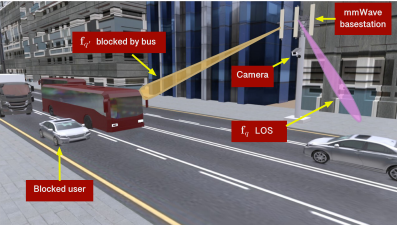
\includegraphics{figures/urban_scenario.png}
    \caption[Urban scenario using vision-based functionality]{Urban scenario using vision-based functionality \cite{Block_predict}.}
    \label{fig:urban_scenario}
\end{figure}

In this context, Computer Vision (CV) is expected to power networks with capabilities beyond traditional telecommunications systems. Using multiple sensors and video cameras, real-time environmental awareness may become a cornerstone for network optimization. For that purpose, state-of-the-art CV algorithms may take charge of tasks related to processing and interpreting visual data while proactively identifying obstacles to prevent signal attenuation and blockage. This convergence of CV and communications represents a promising advancement, fostering heightened responsiveness, adaptability, and overall network performance.


% removing solution from this chapter
%Recognizing these limitations, the 6G paradigm emerges as a response, aiming at paving the way to the evolution from closed systems to open-source implementations. This paradigm envisions a future where the complexity of mobile networks is met with interoperable solutions.

\section{Motivation and Problem}

In the ongoing evolution of mobile networks, successive generations have expanded connectivity capabilities while introducing heightened complexity. This complexity and a growing dependence on closed, proprietary solutions represent a significant challenge to integrating diverse technologies. Acknowledging these limitations becomes imperative, leading to the emergence of the 6G paradigm as a revolutionary response. This paradigm advocates a departure from closed systems to adopting open-source implementations, envisioning a future where mobile networks complexity is met with interoperable solutions. The 6G paradigm stands as a catalyst for change in wireless communications.

However, the 6G paradigm encounters a new layer of complexity imposed by dynamic and moving obstacles,  which may compromise communications in high-frequency bands. This complexity originates from the shorter wavelengths, rendering signals more prone to attenuation when encountering obstacles. Millimeter-wave signals encounter difficulty penetrating solid structures such as walls and buildings, potentially causing signal blockages and dropouts in densely populated urban areas. The presence of vehicular traffic, pedestrians, and other mobile entities in the network's coverage area induces ephemeral shadowing effects, leading to signal blockages and fluctuations that directly impact wireless connectivity reliability. This dynamic scenario poses a considerable challenge to maintaining consistent signal strength and QoS levels, especially in areas with high vehicular or pedestrian density. Effectively addressing the dynamic phenomenon of signal interference from moving obstacles requires adaptive solutions and the implementation of advanced signal tracking, predictive algorithms, and real-time adjustments in network configurations. 

Furthermore, the distinction between Line-of-Sight and Non-Line-of-Sight propagation paths adds to the challenge. LOS paths, with a direct, unobstructed line between the transmitter and receiver, typically offer the most reliable and efficient communication. However, in urban environments, NLOS paths, where signals reflect off buildings or scatter due to obstacles, become prevalent. These NLOS paths introduce additional challenges, such as multipath fading and increased signal attenuation, further exacerbating connectivity issues.

A promising solution to the wireless communications challenges faced in densely populated urban areas lies in obstacle-aware networks, leveraging CV to extract information from video data. By integrating CV algorithms, wireless networks can recognize and proactively overcome the challenges posed by moving obstacles. This approach holds the potential to ensure uninterrupted communications and foster a seamless network experience in urban environments, aligning with the vision set forth by the 6G paradigm.

\section{Objectives}

The main objective of this dissertation was to implement vision-based functionality into a 6G Base Station (gNB), thereby creating a solution for obstacle-aware gNBs. This solution enables a Base Station to autonomously control its placement and configuration based on real-time perception provided by vision-based information.

In order to achieve this goal, specific objectives have been defined:

    \begin{itemize}
    
    \item Implement a mechanism for detecting and tracking objects within the gNB's operational environment, enhancing the gNB's ability to adapt to dynamic environments.
    
    \item Develop a server that extracts relevant information from video. This server should provide information to the mobile network in real time to enhance the gNB's perception and obstacle awareness capabilities.
    
    \item Create a set of messages containing information extracted from the video. This set should be relevant in the context of mobile networks, particularly for use by the gNB.
    
    \item Develop an algorithm, implemented as an xApp, capable of receiving video-extracted information and RAN metrics to determine optimal placement for a RAN node.
      
    \item Validate and evaluate the proposed solution in reference networking scenarios.
    
    \end{itemize}

\section{Contributions}

The main contributions are the following:

    \begin{itemize}
    
    \item The introduction of video-based information into a 5G network, based on O-RAN architecture.
    
    \item A server that extracts relevant information from video feeds, tailored to indoor 5G use case. 
    
    \item A set of structured messages containing video-extracted information. These messages are specifically designed for improving network performance and obstacle management of the gNB.
    
    \item A xApp that processes video-extracted information and RAN metrics to determine optimal placement and configuration for a RAN node. This application enhances the gNB's capabilities by enabling it to make informed decisions based on real-time environmental perception.
    
    \item The validation and evaluation of the performance of the proposed solution in a reference networking scenario. This includes a proof-of-concept for evaluating vision-aided networking solutions.
    
    \end{itemize}


% adjust references to chapters
\section{Document Structure}

This document follows a structured approach. Chapter \ref{ch:state-of-the-art} discusses state-of-the-art and related work containing concepts pertinent to the challenges addressed in this dissertation. Chapter \ref{ch:specs_design_implem} outlines the proposed solution and describes the system's specifications, design choices, and implementation. Chapter \ref{ch:validation} presents the tests conducted to validate and evaluate the implementation of the proposed solution. Finally, Chapter \ref{ch:conclusion} presents synthesized findings, conclusions, and future work.